\documentclass{article}

\usepackage[utf8]{inputenc}
\usepackage[T1]{fontenc}
\usepackage[spanish]{babel}

\usepackage{caratula}
\usepackage{hyperref}
\usepackage{graphicx}
\usepackage{amsmath,amssymb}
\usepackage{minted}
\usepackage{tikz}
\usepackage{tcolorbox}
\usepackage[a4paper, total={7in, 10in}]{geometry}

\setlength{\parindent}{0pt}
\setlength{\parskip}{4pt}

\titulo{Range Queries Con Updates}
\subtitulo{Segment Tree y otras variantes}
\fecha{\today}
\materia{Programación Competitiva II}
\integrante{López Pacholczak, Ulises}{026/23}{ulilopezpacho@gmail.com}

\begin{document}

\maketitle
\tableofcontents
\newpage

\section{Introducción}
Un problema muy interesante en las ciencias de la computación es como poder realizar consultas sobre un arreglo de información de forma eficiente. Por ejemplo, se puede utilizar la técnica de ``Suma de Prefijos'' para poder, con un preprocesamiento de $O(n)$, hacer queries de suma en un rango $[l,r]$ en $O(1)$. O se pueden usar las ``Sparse Tables'' para realizar queries de máximo y mínimo en $O(1)$ con preprocesamiento en $O(n \log n)$

De todas formas, en muchos casos, es necesario ir haciendo modificaciones sobre el arreglo donde se desean hacer las consultas. En esta monografía trabajaremos sobre una estructura de datos llamada ``Segment Tree'' que nos permitirá hacer consultas y actualizaciones en rango de forma eficiente sobre distintas operaciones (suma, máximo, mínimo, entre otras). Además, trabajaremos sobre distintas variantes de esta estructura que nos permitirán obtener ciertas flexibilidades para algunas consultas y actualizaciones.

\section{Segment Tree}
\subsection{Operaciones de la Estructura}

El ``Segment Tree''  es una estructura de datos que nos permitirá realizar queries en rangos y updates en $O(\log n)$ con solo $O(n)$ memoria.

Esta estructura de datos soporta dos operaciones principales:
\begin{itemize}
    \item \textit{query(l: int, r: int): T}, que dado un rango, nos permitirá obtener el resultado de aplicar una cierta operación en el rango $[l,r]$
    \item  \textit{update(pos: int, val: T)} que actualizará el valor de la posición \textit{pos} al indicado en \textit{val}.
\end{itemize}

Ambas operaciones, como fue mencionado anteriormente, tendrán complejidad $O(\log n)$. Además, se puede proponer la operación \textit{build(l: seq<T>)}, que dada un arreglo, construye un Segment Tree en complejidad $O(n)$. De todas formas, esta no suele ser necesaria, ya que se podría construir el mismo inicializándolo con un Segment Tree vacío, y luego aplicando la operación \textit{update}. Lo que sí es necesario es definir $n$, la cantidad de elementos que tendrá el arreglo, previo a realizar las operaciones, ya que se reservará la memoria al inicializar la estructura.

\subsection{Monoides y Segment Tree}

Los ``Segment Trees'' soportan cualquier Monoide. Esto quiere decir que, cualquier estructura algebraica que sea un Monoide podrá ser utilizada con un ``Segment Tree'' para poder realizar queries y updates.

Un Monoide es una estructura algebraica con una operación binaria, que es asociativa y tiene elemento neutro. Un Monoide se lo puede denotar como $(A, \oplus)$ y, en lenguaje matemático formal, cumple las siguientes propiedades:

\begin{itemize}
    \item $\forall a,b,c \in A, (a \oplus b) \oplus c = a \oplus (b \oplus c)$ (es asociativa)
    \item $\exists !e \in A, \forall a \in A, a \oplus e = e \oplus a = a$ (existe neutro)
    \item $\forall a,b \in A, a \oplus b \in A$ (operación cerrada)
\end{itemize}

Entre las operaciones interesantes que pueden utilizarse en un Segment Tree son la suma $(\mathbb{N}, +)$, el máximo $(\mathbb{N}, \max)$, el mínimo $(\mathbb{N}, \min)$, el máximo común divisor $(\mathbb{N}, \gcd)$ entre otras.

\subsection{Representación de la Estructura}

El ``Segment Tree'' es representado en memoria como un Árbol Binario de $2n - 1$ nodos. Para el valor $n$, debe tomarse un número tal que, si llamamos $l$ a la cantidad de elementos del arreglo sobre el cual se desean hacer las consultas, $n = 2^k, k \in \mathbb{N}$, tal que $l \leq 2^{k}$. De esta forma, el árbol binario representado será completo, lo que nos facilitará guardarlo en un arreglo de tal forma que los hijos del nodo $k$ sean $2k$ el hijo izquierdo y $2k + 1$ el hijo derecho, siempre que $1 \leq k < n$. Esto se debe a que, para los nodos entre $n \leq k < 2n$ no tendrán hijos.

Por ejemplo, un ``Segment Tree'' de la siguiente forma (es de suma, pero se puede usar cualquier Monoide):

\begin{center}
\begin{tikzpicture}[scale=0.7]
\draw (0,0) grid (8,1);

\node[anchor=center] at (0.5, 0.5) {5};
\node[anchor=center] at (1.5, 0.5) {8};
\node[anchor=center] at (2.5, 0.5) {6};
\node[anchor=center] at (3.5, 0.5) {3};
\node[anchor=center] at (4.5, 0.5) {2};
\node[anchor=center] at (5.5, 0.5) {7};
\node[anchor=center] at (6.5, 0.5) {2};
\node[anchor=center] at (7.5, 0.5) {6};

\node[draw, circle] (a) at (1,2.5) {13};
\path[draw,thick,-] (a) -- (0.5,1);
\path[draw,thick,-] (a) -- (1.5,1);
\node[draw, circle,minimum size=22pt] (b) at (3,2.5) {9};
\path[draw,thick,-] (b) -- (2.5,1);
\path[draw,thick,-] (b) -- (3.5,1);
\node[draw, circle,minimum size=22pt] (c) at (5,2.5) {9};
\path[draw,thick,-] (c) -- (4.5,1);
\path[draw,thick,-] (c) -- (5.5,1);
\node[draw, circle,minimum size=22pt] (d) at (7,2.5) {8};
\path[draw,thick,-] (d) -- (6.5,1);
\path[draw,thick,-] (d) -- (7.5,1);

\node[draw, circle] (i) at (2,4.5) {22};
\path[draw,thick,-] (i) -- (a);
\path[draw,thick,-] (i) -- (b);
\node[draw, circle] (j) at (6,4.5) {17};
\path[draw,thick,-] (j) -- (c);
\path[draw,thick,-] (j) -- (d);

\node[draw, circle] (m) at (4,6.5) {39};
\path[draw,thick,-] (m) -- (i);
\path[draw,thick,-] (m) -- (j);
\end{tikzpicture}
\end{center}

Será representado en memoria de la siguiente forma:

\begin{center}
\begin{tikzpicture}[scale=0.7]
\draw (0,0) grid (15,1);

\node at (0.5,0.5) {$39$};
\node at (1.5,0.5) {$22$};
\node at (2.5,0.5) {$17$};
\node at (3.5,0.5) {$13$};
\node at (4.5,0.5) {$9$};
\node at (5.5,0.5) {$9$};
\node at (6.5,0.5) {$8$};
\node at (7.5,0.5) {$5$};
\node at (8.5,0.5) {$8$};
\node at (9.5,0.5) {$6$};
\node at (10.5,0.5) {$3$};
\node at (11.5,0.5) {$2$};
\node at (12.5,0.5) {$7$};
\node at (13.5,0.5) {$2$};
\node at (14.5,0.5) {$6$};

\footnotesize
\node at (0.5,1.4) {$1$};
\node at (1.5,1.4) {$2$};
\node at (2.5,1.4) {$3$};
\node at (3.5,1.4) {$4$};
\node at (4.5,1.4) {$5$};
\node at (5.5,1.4) {$6$};
\node at (6.5,1.4) {$7$};
\node at (7.5,1.4) {$8$};
\node at (8.5,1.4) {$9$};
\node at (9.5,1.4) {$10$};
\node at (10.5,1.4) {$11$};
\node at (11.5,1.4) {$12$};
\node at (12.5,1.4) {$13$};
\node at (13.5,1.4) {$14$};
\node at (14.5,1.4) {$15$};
\end{tikzpicture}
\end{center}

Como invariante de representación, los nodos entre $n \leq k < 2n$ serán los nodos originales del arreglo. Esto quiere decir que cuando se llame al procedimiento \textit{update} se actualizará inicialmente el valor de la posición en el arreglo original $i$ en la posición del ``Segment Tree'' $n + i$. Luego, para el resto de los nodos  $1 \leq k < n$, el nodo $k$ contiene el valor de aplicar la operación para todos sus hijos. Es decir, el nodo $k$ tendrá el valor de aplicar la operación en los nodos $2k$ y $2k+1$, luego el nodo $2k$ las aplicará en los nodos $4k$ y $4k + 1$, hasta llegar a la profundiad máxima del arbol. De esta forma, cada nodo guardará los valores de aplicar la operación en un rango $[l,r]$ del arreglo original, siendo ese rango al conjunto de elementos que tiene como hijos (directos o indirectos) en la última capa del arbol, ya que esta equivale al arreglo original.

Para verlo en un ejemplo, en la figura anterior (que es un ``Segment Tree'' con la operación suma), el nodo número $3$, con valor $17$, contiene la suma de sus dos nodos hijos (nodos $6$ y $7$ con valores $9$ y $8$ respectivamente), y representa la suma en el rango del arreglo original $[4,7]$, ya que contiene como hijos en la última capa a los nodos $12$, $13$, $14$ y $15$ equivalentes en el arreglo original (restando $n$ se obtiene la equivalencia) a las posiciones $4$, $5$, $6$ y $7$ respectivamente.

\subsection{Las Operciones}

Para implementar las operaciones, se puede hacer tanto con un enfoque iterativo o recursivo. El enfoque recursivo suele ser mucho más claro, aunque el enfoque iterativo suele ser más útil y fácil de programar en competencias. Por eso, comencemos describiendo el algoritmo recursivo, y veamos su código. Trabajaremos sobre el caso de suma, pero se puede fácilmente generalizar para cualquier otro Monoide.

\subsubsection{Enfoque Recusivo}

Para obtener la suma dado un ``Segment Tree'' válido, definiremos una función auxiliar \textit{query(a: int, b: int, k: int, x: int, y: int)} que nos permitirá obtener la suma en el rango. \textit{a} y \textit{b} son el rango de la forma inclusiva-inclusiva sobre el cual nosotros queremos hacer la consulta. Luego, \textit{k} indica el nodo sobre el que estamos parados, y \textit{x} e \textit{y} siempre van a mantener el rango que abarca a ese nodo. Incialmente, por eso, la función siempre va a ser llamada con los parámetros \textit{query(l, r, 1, 0, n-1)}.

La función recursiva, entonces, evalúa los siguientes casos:
\begin{itemize}
    \item Si el rango está fuera del intervalo que representa ese nodo es vacío (es decir, el rango $[a,b]\cap[x,y] = \emptyset$), se debe devolver el elemento neutro. En caso de la suma, el $0$.
    \item Si el rango está totalmente contenido dentro del intervalo, debemos retornar el valor en $segTree[k]$, ya que ahí se encuentra la suma del rango $[x,y]$.
    \item Si el rango está parcialmente contenido, entonces se recurre a los dos subárboles izquierdo y derecho. Esto se repetirá hasta caer en alguno de los dos casos anteriores, que siempre ocurren al llegar al último piso del árbol.
\end{itemize}

Esto se puede implementar de la siguiente forma:

\begin{minted}{c++}
int query(int a, int b, int k, int x, int y) {
    if (b < x || a > y) return 0;
    if (a <= x && y <= b) return segTree[k];
    int d = (x+y)/2;
    return query(a,b,2*k,x,d) + query(a,b,2*k+1,d+1,y);
}
\end{minted}

Puede pensarse que esto puede tener una complejidad de $O(n)$, ya que se podría llamar muchas veces al subarbol de forma recursiva. Pero no es así, ya que, en el peor de los casos, se puede ver que para cada capa del Arbol Binario a lo sumo se van a tener cuatro llamadas a la función \textit{query}. Esto se debe a que el intervalo sobre el cual uno hace las preguntas es continuo. Por ende, como el Arbol Binario tiene profundidad $\log_2 n$, la complejidad de este algoritmo será $O(\log n)$.

Ahora, vayamos a analizar la operación de \textit{update}. Al igual que en el caso anterior, nombraremos una función auxiliar \textit{update(pos: int, k: int, x: int, y: int, val: int)} que indicará en \textit{pos} la posición del arreglo original que será modificada, \textit{k}, \textit{x} e \textit{y} representan lo mismo que en el caso anterior (el nodo actual, el principio y el final del rango que representa ese nodo respectivamente), y por último \textit{val}, que es el nuevo valor a asignar. La función se llamará inicialmente de la siguiente forma: \textit{update(pos, 1, 0, n-1, val)}.

La función evalúa los siguientes casos:
\begin{itemize}
    \item Si estoy en el útlimo nivel del Arbol Binario (entonces $x=y$), asigno $val$ a esa posición y retorno ya que no hay más capas a ser recorridas del arbol.
    \item Caso contrario, reviso si $pos$ está en el subarbol izquierdo o derecho, chequeando si es mayor o menor al promedio de $x$ e $y$. Enonces, recurro al subarbol que corresponda, y una vez actualizado ese arbol (al salir de todas las llamadas recursivas), actualizo mi valor aplicando la operación correspondiente sobre los dos nodos hijos.
\end{itemize}
Esto se puede implementar de la siguiente forma:
\begin{minted}{c++}
void update(int pos, int k, int x, int y, int val) {
    if (x == y) { segTree[k] = val; return; }
    int d = (x + y) / 2;
    if (pos <= d) update(pos, k*2, x, d, val);
    else update(pos, k*2+1, d+1, y, val);
    segTree[k] = segTree[k*2] + segTree[k*2+1];
}
\end{minted}
Nuevamente, la complejidad de esta operación es $O(\log n)$ ya que se recorre cada una de las capas del Arbol Binario Completo una sola vez.

\subsubsection{Enfoque Iterativo}

Analizaremos este enfoque de forma más breve, ya que no es tan importante comprenderlo (con el enfoque recursivo alcanzará para comprender el tema). 

La operación \textit{query(a: int, b: int)} lo que hace es ir iterando capa a capa del Arbol Binario, desde la inferior hasta la superior, siempre manteniendo $a$ en el borde izquierdo del intervalo y $b$ en el borde derecho del mismo. Inicialmente, se encuentra en el rango $[a+n, b+n]$ ya que de $n$ hasta $2n$  es donde se encuentra el arreglo original. Cada paso que se mueve a una capa superior, los valores de los nodos que no pertenezcan a la capa del arbol son agregados a la suma, y ese índice $a$ o $b$ pasa a apuntar a otro que es candidato a estar dentro del rango. Luego, una vez que se  ``cruzan'' los dos punteros, significa que el rango ya fue abarcado en su totalidad, por lo que en $s$ ya se encuentra en la respuesta.

\begin{minted}{c++}
int query(int a, int b) {
    a += n; b += n;
    int s = 0;
    while (a <= b) {
        if (a%2 == 1) s += tree[a++];
        if (b%2 == 0) s += tree[b--];
        a /= 2; b /= 2;
    }
    return s;
}
\end{minted}
La complejidad de esta operación es $O(\log n)$.

Para la operación \textit{update(k: int, x: int)}, actualiza a la posición $k$ del arreglo original con el valor $x$. Luego, itera todos los padres del nodo modificado recomputando la suma de cada uno de ellos. El código es sencillo, y es el siguiente:

\begin{minted}{c++}
void update(int k, int x) {
    k += n, tree[k] = x;
    for (k /= 2; k >= 1; k /= 2) {
        tree[k] = tree[2*k]+tree[2*k+1];
    }
}
\end{minted}

La complejidad será $O(\log n)$ también.

\subsection{Problemas Clásicos}

Los siguientes problemas requieren únicamente la implementación de esta estructura de datos. El código de las soluciones se encontrará disponible en el Anexo de esta monografía.

\subsubsection{CSES 1648 - Dynamic Range Sum Queries}

Link al Problema: \href{https://cses.fi/problemset/task/1648}{https://cses.fi/problemset/task/1648}

\begin{tcolorbox}
Dado un arreglo de $n$ enteros, tu tarea es procesar $q$ queries de los siguientes tipos:
\begin{enumerate}
    \item Actualizar el valor en la posición $k$ a un valor $u$
    \item Cual es la suma de los valores en el rango $[a,b]$?
\end{enumerate}
Tanto $q$ y $n$ pueden ser como máximo $2*10^5$
\end{tcolorbox}

Para resolver este problema, solo se necesita implementar la estructura de datos del ``Segment Tree'', ya que la suma es un monoide. Dejaré tanto la solución recursiva como la iterativa.

\subsubsection{CSES 1649 - Dynamic Range Minimum Queries}

Link al Problema: \href{https://cses.fi/problemset/task/1648}{https://cses.fi/problemset/task/1648}

\begin{tcolorbox}
Dado un arreglo de $n$ enteros, tu tarea es procesar $q$ queries de los siguientes tipos:
\begin{enumerate}
    \item Actualizar el valor en la posición $k$ a un valor $u$
    \item Cual es el mínimo de los valores en el rango $[a,b]$?
\end{enumerate}
Tanto $q$ y $n$ pueden ser como máximo $2*10^5$
\end{tcolorbox}

Este problema lo resolveré utilizando un código genérico de ``Segment Tree'' que puede ser utilizado para cualquier Monoide. Para esto, es solo necesario redefinirse \textit{Node} que tiene una función \textit{identity()}, que devuelve la identidad del Monoide, y el \textit{operator>{}>}, que actúa al aplicar la operación entre dos nodos. En este caso, lo implementé con el mínimo, ya que es el lo que pedía el problema.


\section{Técnicas Adicionales sobre Segment Tree}

En esta parte aprenderemos algunas técnicas que nos permitirán aprovechar más esta estructura de datos.

\subsection{Búsqueda Binaria}

Además de la operación \textit{query} que trabajamos anteriormente, podemos utilizar búsqueda binaria para poder encontrar elementos dentro del arreglo sobre el cual se hacen consultas, bajo un cierto criterio. Por ejemplo, podemos determinar la primera posición $k$ que es menor o igual a un cierto valor $x$ en el caso de un ``Segment Tree'' de mínimos, o también se puede encontrar el mínimo prefijo que sume al menos $x$ para el caso de que se esté trabajando sobre la suma. Para poder aplicar esta técnica, uno comienza parado en el nodo raíz, y observando los valores del nodo padre del subárbol izquierdo y derecho, toma una decisión. De esta forma, se estaría aplicando una forma de recorrer el árbol similar a como se hace en un Árbol Binario de Búsqueda, pero sin mantener la invariante que tienen estos tipos de árboles. Veamos un ejemplo para entender más fácilmente esto.

\subsubsection{CSES 1143 - Hotel Queries}

Link al problema: \href{https://cses.fi/problemset/task/1143}{https://cses.fi/problemset/task/1143}
\begin{tcolorbox}
Hay $n$ hoteles en una calle. Para cada hotel conoces el número de habitaciones libres. Tu tarea es asignar habitaciones de hotel para grupos de turistas. Todos los miembros de un grupo quieren alojarse en el mismo hotel.

Los grupos llegarán a usted uno tras otro y usted sabrá para cada grupo la cantidad de habitaciones que necesita. Siempre asignas un grupo al primer hotel que tenga suficientes habitaciones. Después de esto, el número de habitaciones libres en el hotel disminuye.

Para cada grupo de turistas, imprima el número del hotel al que fueron asignados.
\end{tcolorbox}

Para resolver el problema, vamos a usar el ``Segment Tree''  de máximos como una estructura para hacer Binary Search. La idea es encontrar el primer hotel que tenga suficientes habitaciones para el grupo de turistas en $O(\log n)$. Como base, utilizaremos un ``Segment Tree'' de máximos, que se realizará sobre el arreglo base de habitaciones disponibles de cada uno de los hoteles. Los hoteles estarán ordenados según cuál estará primero. Esto nos será de utilidad para hallar el primer hotel con habitaciones suficientes haciendo búsqueda binaria.

Para cada grupo de turistas, partimos desde el primer nodo (la raíz). Nos moveremos hacia el subárbol izquierdo si su padre contiene un número mayor o igual a la cantidad de habitaciones que necesitamos, o al de la derecha si el nodo contiene un número menor. De esta forma, cuando arribemos a la última capa del Árbol Binario Completo, nos encontraremos en el primer hotel que tenga la suficiente cantidad de habitaciones. Esto se debe a que siempre que había algún hotel con al menos esta cantidad de habitaciones disponibles, nos fuimos en la dirección con índice menor del arreglo. De esta forma, la respuesta va a ser $k-n$, siendo $k$ el nodo de la última capa al cual llegamos. También, cabe aclarar que si no hay habitaciones suficientes en ningún hotel para este grupo (que alcanza con verificar que la raíz tenga un número más chico que la cantidad de habitaciones requerida por el grupo), la función devolverá $0$.

El código para resolver este problema se encuentra en el Anexo. En este, se planteó una función \textit{occupy} que busca el hotel a ocupar, ocupa las habitaciones y retorna el hotel que se ocupó, según lo solicitado por el enunciado. Como cada llamada a esta función tiene complejidad $O(\log n)$, la complejidad total del ejercicio es $O(n \log n)$. De esta forma, trabajamos cómo se puede usar Binary Search sobre un ``Segment Tree''.

\subsection{Compresión de Coordenadas}

Esta es una técnica muy utilizada en Programación Competitiva cuando se cumplen las siguientes hipótesis:
\begin{itemize}
    \item Uno debe utilizar una estructura de datos basada en arreglos.
    \item Los índices pueden llegar a valores muy grandes.
    \item Se saben de antemano con cuales índices uno desea trabajar, es decir, cuáles índices son relevantes para la resolución del problema.
\end{itemize}
La idea de esto es tomar el conjunto de índices $C_i = \{I_1, I_2, ..., I_n\}$ que se utilizarán en el caso de prueba (que generalmente se pueden obtener analizando el input), y luego se define una función biyectiva $f(i)$ que mapea cada uno de los índices a un número entre $[0,n-1]$ siendo $n = \#C_i$ (cantidad de elementos del conjunto) manteniendo que, para dos índices $i,j\in C_i$, con $i\neq j$, si $i < j \implies f(i) < f(j)$. De esta forma, según la cantidad de distintos valores que reciba el input, indicará cuántos elementos tendrá el mapeo de índices. De esta forma, se podrán volver a utilizar distintas estructuras sobre arreglos que con tamaños muy grandes se dificultaba, como es el ``Segment Tree''.

Desde el punto de vista implementativo, para poder mapear desde un índice $I_n$ a $f(I_n)$ se puede utilizar un \textit{map} o un \textit{unordered\_map}. Para mapear la vuelta, es decir desde $f(I_n)$ a $I_n$ (lo que se puede hacer porque la funcion es biyectiva), se puede usar un \textit{array}. Ahora, veamos un problema para ver cómo se aplica esto.

\subsubsection{CSES 1144 - Salary Queries}
Link al Problema: \href{https://cses.fi/problemset/task/1144}{https://cses.fi/problemset/task/1144}

\begin{tcolorbox}
Una compañía tiene $n$ empleados con ciertos salarios. Tu tarea es procesar salarios, pudiendo preguntar cuales eran los salarios de los empleados en un rango, y actualizar el salario de un empleado. Los salarios pueden ir entre $0$ y $10^9$.
\end{tcolorbox}

El gran problema que tiene este ejercicio es que los salarios pueden ser hasta $10^9$, por lo que si queremos guardar un Segment Tree en el que cada posición guarde cuántas personas tienen ese salario (para hacer una query de rangos) requeriríamos muchísima memoria. Es por eso que debemos recurrir a compresión de coordenadas. Lo que debemos hacer es leer todo el input de entrada, y guardar todos los posibles valores de los salarios actuales y futuros en un arreglo, al cual llamaremos $compresion$ Luego, se puede mapear, una vez ordenado el arreglo y eliminado los repetidos, cada valor a un índice entre $[0, c-1]$ siendo $c$ la cantidad de salarios distintos. Luego, podemos armar un \textit{map} que mapee cada salario posible a su posición en ese arreglo creado anteriormente.

Para poder procesar las queries, utilizaremos un ``Segment Tree'' de longitud igual (o su potencia de $2$ más grande y cercana) a la cantidad de elementos de la lista de compresión de coordenadas (es decir, con la cantidad de salarios distintos). Cada posición del arreglo indica cuántas personas tienen el salario $compresion[i]$, siendo $i$ el índice en el arreglo sobre el cual se realizan las consultas. Entonces, en el caso que se nos pida actualizar un salario, simplemente debemos restarle $1$ a la posición con el salario anterior, y sumarle $1$ al nuevo salario. Por ende, es de utilidad ir guardando en otro arreglo el valor del salario actual para un empleado e ir actualizándolo a medida que se van realizando los cambios.

Para realizar las consultas, entonces, se puede hacer una búsqueda binaria sobre el arreglo $compresion$ para encontrar los índices en el arreglo de consultas sobre los cuales llamar al ``Segment Tree'', o, si se agregó a $compresion$ los valores donde se hacen las consultas, se puede utilizar el \textit{map} de salarios a índice en el arreglo de consultas para saber que valores pasarle al método \textit{query} del ``Segment Tree''. De esta forma, pudimos resolver el problema con complejidad $O(n \log n)$, ya que cada consulta o actualización va a tener complejidad $O(\log n)$.

En el Anexo se encuentra disponible el código que resuelve este problema. Este es un ejemplo de como se puede usar compresión de coordenadas para utilizar estructuras de datos sobre arreglos.

\subsection{Segment Trees Dinámicos}

Existen algunos problemas donde uno debe utilizar esta estructura de datos sobre rangos con números muy grandes, pero uno no posee de entrada todos los valores sobre los cuales se deben realizar las consultas y actualizaciones, como es en el caso anterior. Este tipo de problemas es conocido como problemas ``online'', y suelen requerir responder una consulta o actualización antes de recibir la siguiente. Si nosotros alocáramos toda la memoria de entrada y representáramos el ``Segment Tree'' como hicimos anteriormente, nos quedaríamos sin memoria. Pero, para subsanar esto, podemos recurrir a la memoria dinámica y almacenar solo los nodos que tengan valores interesantes para nosotros.

De esta forma, la implementación del ``Segment Tree'' es muy similar a la recursiva que trabajamos anteriormente, a diferencia que cada nodo del árbol no va a ser representado más como una posición en un arreglo, sino más bien va a ser un \textit{struct} que contenga un puntero tanto hacia su hijo izquierdo como su hijo derecho. Será \textit{nullptr} si uno no tendrá más hijos, o si una rama no tiene ningún valor seteado. El \textit{struct} se vería de la siguiente forma:

\begin{minted}{c++}
using tint = long long;
struct Node {
  tint value;
  Node *left, *right;
  Node(tint value): value(value) {}
  Node(): value(0) {}
};
\end{minted}

De esta forma, en la operación \textit{query}, antes de recurrir a cada uno de los hijos, debemos chequear si estos nodos existen. Si no existen, es como si estos tuvieran el valor identidad para el Monoide con el que se está trabajando. Para la operación \textit{update}, en cada paso se debe chequear si el nodo que contiene el valor a actualizar existe. En caso de que que no exista, es decir, que hacia la dirección que se quiere realizar la actualización sea \textit{nullptr}, debe crearse el nodo y luego recurrir a ese subárbol. El proceso finalizará cuando se llegue a la última capa del árbol, donde el nodo represente al elemento del arreglo sobre el cual se hacían originalmente las consultas.

Cabe aclarar que es necesario al inicializar la estructura indicar el máximo $n$ que esta puede llegar a soportar, ya que esto indica la profundidad que va a tener el árbol al momento de realizar las consultas. Por ejemplo, si $n=10^9$, el árbol tendrá una profundidad de $\log_2(10^9)\approx30$. Por ultimo, también hay que recordar que en C++ se debe liberar la memoria una vez destruida la estructura de datos. Aunque en programación competitiva no es totalmente necesario realizarlo (ya que el juez corre cada caso de prueba por separado o nos da mucha memoria disponible), es una buena práctica en el mundo del del desarrollo de software.

\subsubsection{CSES 1144 - Salary Queries - Segment Tree Dinámico}

Link al problema: \href{https://cses.fi/problemset/task/1144}{https://cses.fi/problemset/task/1144}

Este problema, trabajado en la sección anterior, puede también ser resuelto utilizando un ``Segment Tree Dinámico''. Simplemente se crea esta estructura con el máximo $n=10^9$ y se puede llamar a las funciones \textit{update} y \textit{query} con los valores indicados por el enunciado. Al igual que en el desarrollo anterior, cada posición del arreglo original (que en este caso está implícito al usar una estructura dinámica) contiene la cantidad de personas que tienen ese salario. Luego, la estructura es modelada con la operación suma, y en $O(\log n)$ podemos saber cuántas personas tienen un salario entre $a$ y $b$, dados por cada una de las consultas. Para la actualización de los valores, se le resta $1$ a la posición que representa al salario que el empleado tenía anteriormente, y se le suma $1$ al nuevo salario. De esta forma, quedaría modelado el problema. En el Anexo se encuentra el código para esta solución.

\section{Lazy Propagation Segment Tree}

Ahora, imaginemos que no solo nos interesa realizar actualizaciones de un único valor, sino que nos interesa hacer actualizaciones de un rango $[a,b]$. Si uno desea hacer este tipo de actualizaciones y solo interesa hacer una query del valor de una celda únicamente, se puede hacer usando un ``Segment Tree'' clásico almacenando la información como una arreglo de diferencias. Pero, esto nos limita también a no hacer queries en rangos. Es por eso que el ``Segment Tree'' con propagación perezosa nos va a permitir hacer actualizaciones en rango en $O(\log n)$ y también consultas en rango en $O(\log n)$. ¡La misma complejidad que un Segment Tree tradicional! De todas formas, tiene contras, ya que utiliza más memoria que el ``Segment Tree'' clásico y además no se puede usar para cualquier Monoide, sino que solo para operaciones que se puedan componer. A continuación, analizaremos el funcionamiento de esta estructura.

\subsection{Operaciones de la Estructura}

El ``Lazy Segment Tree'' soportará las siguientes dos operaciones principales, ambas con complejidad en $O(\log n)$:
\begin{itemize}
    \item \textit{query(l: int, r: int): T}, que dado un rango, nos permitirá obtener el resultado de aplicar una cierta operación en el rango $[l,r]$
    \item  \textit{update(l: int, r: int, val: T)} que actualizará los valores en el rango $[l,r]$ con el valor indicado en \textit{val}. Se pueden definir distintas operaciones de actualización. Por ejemplo, en un ``Lazy Segment Tree'' de suma se puede crear un \textit{update} para setear un segmento a un cierto valor $val$, u otra operación para incrementar ese segmento por $val$. Lo que se debe cumplir es que las operaciones se puedan componer.
\end{itemize}

Cabe aclarar que estas estructuras de datos no funcionan con todos los Monoides. Solo funcionan con operaciones que además de ser Monoides, se deben poder componer para poder ser aplicadas todas juntas. Por ejemplo, si se aplica la operación suma a un nodo con valores $2$, $4$ y $6$ es equivalente a aplicar una sola vez la operación sumar $12$. Por ende, no habría problema de utilizar esta estructura de datos en este caso.

\subsection{Representación de la Estructura}

La estructura se puede representar utilizando un arreglo de \textit{nodos}, con las mismas consideraciones que un ``Segment Tree'' clásico. Lo que hay que tener en cuenta es que cada \textit{Nodo} tendrá no solo el valor actual de este nodo, sino que también contendrá más valores que nos permitirán hacer una propagación perezosa. Esto se entenderá más al analizar la implementación de las operaciones.

\subsection{Las Operaciones}

Para poder implementar las operaciones de un ``Lazy Segment Tree'', es más cómodo aplicar un enfoque recursivo. Para facilitar la explicación, trabajaré cada uno de los algoritmos dando como ejemplo al ``Lazy Segment Tree'' de suma, que nos permitirá hacer una consulta en rango de la suma en $[l,r]$ y una actualización en $[l,r]$ que consiste en incrementar o decrementar cada nodo de ese rango por un valor $val$. En este caso, cada \textit{Nodo} almacenará dos valores: la suma de los elementos del subárbol (llamado a partir de ahora $sum$) y el valor por el cuál va a ser incrementado o decrementado todo el subárbol (el cual será llamado $lazy$). Veamos cada una de las operaciones, en este caso comenzando por \textit{update} y luego yendo por \textit{query}.

La operación de \textit{update} irá recorriendo de forma recursiva cada subárbol según el rango que desea ser actualizado. Para ello, nos definiremos una función auxiliar muy similar a la del ``Segment Tree'' clásico, con los siguientes parámetros: \textit{update(a: int, b: int, val: int, k: int, l: int, r: int)}, con $[a,b]$ el rango a actualizar, $val$ el valor a aplicar, $k$ el número de nodo actual que representa el rango $[l,r]$ del arreglo original. La función aplicará el siguiente algoritmo:

\begin{itemize}
    \item Si el rango $[l,r]$ está afuera del rango del nodo $[a,b]$, es decir $[a,b]\cap[x,y] = \emptyset$, retornar, ya que no se debe hacer nada.
    \item Si el rango $[a,b]$ está totalmente contenido dentro de $[l,r]$, es decir $[a,b]\cap[l,r] = [a, b]$, setear el valor $lazy$ y retornar. En el caso de la suma, sería incrementar el valor $lazy$ por $val$. Eso significa que en $lazy$ quedará una operación pendiente a aplicar en los nodos inferiores, que se hará cuando sea necesario, ya que teniendo la suma de los subárboles en $suma$ y este valor $lazy$ se puede deducir cuál va a ser el valor total del nodo, mediante la \textit{evaluación} del mismo.
    \item Si el rango $[l,r]$ está parcialmente contenido en $[a,b]$, que es cuando $[a,b]\cap[x,y]\neq\emptyset$, se deberá propagar los valores $lazy$ a los subárboles izquierdo y derecho, y borrar del nodo ese valor (setearlo a $0$ en el caso de la suma). Con propagar se refiere a aplicar una función que le indique a los subárboles qué conjunto de operaciones deben aplicar. En el caso de la suma con operación de incrementar en $val$, este paso consiste en simplemente en sumar el valor $lazy$ a cada uno de los valores $lazy$ de sus subárboles. Luego, se llama a actualizar a cada uno de estos de forma recursiva, similar a como se hacía en el \textit{query} del ``Segment Tree'' clásico.
    \item Por último, si se cayó en el tercer caso de los anteriores, se actualiza el valor de este nodo, evaluando cada uno de los nodos hijos. Para el caso de la suma, el resultado de evaluar los hijos se guardará en $sum$.
\end{itemize}

Este algoritmo, al tener un esquema muy similar al \textit{update} de la estructura de datos original, tiene una complejidad de $O(\log n)$. Además, cabe aclarar que la función de evaluación para un nodo para el caso de la suma será $eval(k) = suma + lazy \times (r-l+1)$, con $(r-l+1)$ la cantidad de hijos que tiene este nodo. Esta operación hace sentido ya que $lazy \times (r-l+1)$ es equivalente a el resultado que tendría el nodo de aplicar esa operación perezosa a cada uno de los elementos en el rango $[l,r]$. Y además, se le agrega $suma$, que indica los valores de suma para cada uno de los subárboles izquierdo y derecho.

Por ejemplo, dado un ``Lazy Segment Tree'' genérico, sumarle $2$ al rango $[a,b]$ del gráfico resultaría en el siguiente ``Lazy Segment Tree'':

\begin{center}
\begin{tikzpicture}[scale=0.7]
\fill[color=gray!50] (5,0) rectangle (6,1);
\draw (0,0) grid (16,1);

\foreach \x  [count=\pos from 0] in {5,8,6,3,2,9,2,6,7,1,7,5,6,2,3,2}{
  \pgfmathsetmacro{\posp}{\pos+0.5}
  \node[anchor=center] at (\posp, 0.5) {\x};
}

%\node[anchor=center] at (0.5, 0.5) {5};
%\node[anchor=center] at (1.5, 0.5) {8};
%\node[anchor=center] at (2.5, 0.5) {6};
%\node[anchor=center] at (3.5, 0.5) {3};
%\node[anchor=center] at (4.5, 0.5) {2};
%\node[anchor=center] at (5.5, 0.5) {9};
%\node[anchor=center] at (6.5, 0.5) {2};
%\node[anchor=center] at (7.5, 0.5) {6};
%\node[anchor=center] at (8.5, 0.5) {7};
%\node[anchor=center] at (9.5, 0.5) {1};
%\node[anchor=center] at (10.5, 0.5) {7};
%\node[anchor=center] at (11.5, 0.5) {5};
%\node[anchor=center] at (12.5, 0.5) {6};
%\node[anchor=center] at (13.5, 0.5) {2};
%\node[anchor=center] at (14.5, 0.5) {3};
%\node[anchor=center] at (15.5, 0.5) {2};
%
\node[draw, circle] (a) at (1,2.5) {13/0};
\path[draw,thick,-] (a) -- (0.5,1);
\path[draw,thick,-] (a) -- (1.5,1);
\node[draw, circle,minimum size=32pt] (b) at (3,2.5) {9/0};
\path[draw,thick,-] (b) -- (2.5,1);
\path[draw,thick,-] (b) -- (3.5,1);
\node[draw, circle,minimum size=32pt] (c) at (5,2.5) {11/0};
\path[draw,thick,-] (c) -- (4.5,1);
\path[draw,thick,-] (c) -- (5.5,1);
\node[draw, circle,fill=gray!50,minimum size=32pt] (d) at (7,2.5) {8/2};
\path[draw,thick,-] (d) -- (6.5,1);
\path[draw,thick,-] (d) -- (7.5,1);
\node[draw, circle,minimum size=32pt] (e) at (9,2.5) {8/0};
\path[draw,thick,-] (e) -- (8.5,1);
\path[draw,thick,-] (e) -- (9.5,1);
\node[draw, circle] (f) at (11,2.5) {12/0};
\path[draw,thick,-] (f) -- (10.5,1);
\path[draw,thick,-] (f) -- (11.5,1);
\node[draw, circle,fill=gray!50,minimum size=32pt] (g) at (13,2.5) {8/2};
\path[draw,thick,-] (g) -- (12.5,1);
\path[draw,thick,-] (g) -- (13.5,1);
\node[draw, circle,minimum size=32pt] (h) at (15,2.5) {5/0};
\path[draw,thick,-] (h) -- (14.5,1);
\path[draw,thick,-] (h) -- (15.5,1);
%
\node[draw, circle] (i) at (2,4.5) {22/0};
\path[draw,thick,-] (i) -- (a);
\path[draw,thick,-] (i) -- (b);
\node[draw, circle] (j) at (6,4.5) {23/0};
\path[draw,thick,-] (j) -- (c);
\path[draw,thick,-] (j) -- (d);
\node[draw, circle,fill=gray!50] (k) at (10,4.5) {20/2};
\path[draw,thick,-] (k) -- (e);
\path[draw,thick,-] (k) -- (f);
\node[draw, circle] (l) at (14,4.5) {17/0};
\path[draw,thick,-] (l) -- (g);
\path[draw,thick,-] (l) -- (h);
%
\node[draw, circle] (m) at (4,6.5) {45/0};
\path[draw,thick,-] (m) -- (i);
\path[draw,thick,-] (m) -- (j);
\node[draw, circle] (n) at (12,6.5) {45/0};
\path[draw,thick,-] (n) -- (k);
\path[draw,thick,-] (n) -- (l);
%
\node[draw, circle] (o) at (8,8.5) {90/0};
\path[draw,thick,-] (o) -- (m);
\path[draw,thick,-] (o) -- (n);
%
\path[draw=red,thick,-stealth,line width=2pt] (o) -- (m);
\path[draw=red,thick,-stealth,line width=2pt] (o) -- (n);
%
\path[draw=red,thick,-stealth,line width=2pt] (m) -- (j);
\path[draw=red,thick,-stealth,line width=2pt] (j) -- (c);
\path[draw=red,thick,-stealth,line width=2pt] (j) -- (d);
\path[draw=red,thick,-stealth,line width=2pt] (c) -- (5.5,1);
%
\path[draw=red,thick,-stealth,line width=2pt] (n) -- (k);
\path[draw=red,thick,-stealth,line width=2pt] (n) -- (l);
%
\path[draw=red,thick,-stealth,line width=2pt] (l) -- (g);
%
\node at (5.5,-0.75) {$a$};
\node at (13.5,-0.75) {$b$};

\end{tikzpicture}
\end{center}

Ahora, analicemos la función \textit{query} para el ``Lazy Segment Tree''. Esta operación, nuevamente, tendrá una función auxuliar, que es similar a la de ``Segment Tree'' tradicional: \textit{query(a: int, b: int, k: int, x: int, y: int)} con $[a,b]$ el rango sobre el cual se quiere hacer la \textit{query}, $k$ el número de nodo actual y el rango $[l,r]$, el rango que representa el nodo $k$ en el arreglo original. El algoritmo sería de la siguiente forma:

\begin{itemize}
    \item Si el rango $[l,r]$ está afuera del rango del nodo $[a,b]$, es decir $[a,b]\cap[x,y] = \emptyset$, retornar el valor identidad, como en el caso de la suma el $0$ ya que no hay valores que estén en el rango solicitado para ese nodo.
    \item Si el rango $[a,b]$ está totalmente contenido en el nodo, es decir $[a,b]\cap[l,r] = [a, b]$, retornar el valor resultante de \textit{evaluar} el nodo con la función definida para el problema. En el caso de la suma, con la función descripta anteriormente. Esto devolverá el valor que tiene el rango representado por el nodo al aplicar la operación.
    \item Si no ocurre ninguno de los dos casos anteriores, es decir que el nodo está parcialmente contenido en el intervalo a buscar, se debe realizar un paso de propagación idéntico al momento de actualizar. Esto se debe a que nosotros vamos a hacer consultas en los dos subárboles, y para ello necesitamos que todas las actualizaciones ya hayan sido hechas para cada uno de los subárboles al momento de consultarlos. Esto se logra a través del paso de propagación, que informará a los nodos hijos los valores que estos van a tener. Al igual que en el caso anterior, al momento de propagar las actualizaciones, se deben borrar de este nodo, ya que hasta este punto las operaciones fueron aplicadas.
    \item Luego, si se cayó en el caso anterior, se llama recursivamente a \textit{query} en cada uno de los dos hijos. Esto nos va a dar la información que se debe devolver para esta consulta. De todas formas, resta actualizar el valor actual del nodo, ya que se propagó la actualización pero no se aplicó el resultado de realizarla en sus hijos. Por ende, se evalúan los nodos hijos y se aplica la operación al evaluarlos. Luego, finalmente, se retornan los valores.
\end{itemize}

Por ejemplo, dado un ``Lazy Segment Tree'', consultar al rango $[a,b]$ produciría una propagación en el árbol de la siguiente forma (además de retornar la suma):

\begin{center}
\begin{tikzpicture}[scale=0.7]
\draw (0,0) grid (16,1);

\node[anchor=center] at (0.5, 0.5) {5};
\node[anchor=center] at (1.5, 0.5) {8};
\node[anchor=center] at (2.5, 0.5) {6};
\node[anchor=center] at (3.5, 0.5) {3};
\node[anchor=center] at (4.5, 0.5) {2};
\node[anchor=center] at (5.5, 0.5) {9};
\node[anchor=center] at (6.5, 0.5) {2};
\node[anchor=center] at (7.5, 0.5) {6};
\node[anchor=center] at (8.5, 0.5) {7};
\node[anchor=center] at (9.5, 0.5) {1};
\node[anchor=center] at (10.5, 0.5) {7};
\node[anchor=center] at (11.5, 0.5) {5};
\node[anchor=center] at (12.5, 0.5) {6};
\node[anchor=center] at (13.5, 0.5) {2};
\node[anchor=center] at (14.5, 0.5) {3};
\node[anchor=center] at (15.5, 0.5) {2};

\node[draw, circle] (a) at (1,2.5) {13/0};
\path[draw,thick,-] (a) -- (0.5,1);
\path[draw,thick,-] (a) -- (1.5,1);
\node[draw, circle,minimum size=32pt] (b) at (3,2.5) {9/0};
\path[draw,thick,-] (b) -- (2.5,1);
\path[draw,thick,-] (b) -- (3.5,1);
\node[draw, circle,minimum size=32pt] (c) at (5,2.5) {11/0};
\path[draw,thick,-] (c) -- (4.5,1);
\path[draw,thick,-] (c) -- (5.5,1);
\node[draw, circle,minimum size=32pt] (d) at (7,2.5) {8/2};
\path[draw,thick,-] (d) -- (6.5,1);
\path[draw,thick,-] (d) -- (7.5,1);
\node[draw, circle,minimum size=32pt] (e) at (9,2.5) {8/2};
\path[draw,thick,-] (e) -- (8.5,1);
\path[draw,thick,-] (e) -- (9.5,1);
\node[draw, circle,fill=gray!50,] (f) at (11,2.5) {12/2};
\path[draw,thick,-] (f) -- (10.5,1);
\path[draw,thick,-] (f) -- (11.5,1);
\node[draw, circle,fill=gray!50,minimum size=32pt] (g) at (13,2.5) {8/2};
\path[draw,thick,-] (g) -- (12.5,1);
\path[draw,thick,-] (g) -- (13.5,1);
\node[draw, circle,minimum size=32pt] (h) at (15,2.5) {5/0};
\path[draw,thick,-] (h) -- (14.5,1);
\path[draw,thick,-] (h) -- (15.5,1);

\node[draw, circle] (i) at (2,4.5) {22/0};
\path[draw,thick,-] (i) -- (a);
\path[draw,thick,-] (i) -- (b);
\node[draw, circle] (j) at (6,4.5) {23/0};
\path[draw,thick,-] (j) -- (c);
\path[draw,thick,-] (j) -- (d);
\node[draw, circle] (k) at (10,4.5) {28/0};
\path[draw,thick,-] (k) -- (e);
\path[draw,thick,-] (k) -- (f);
\node[draw, circle] (l) at (14,4.5) {17/0};
\path[draw,thick,-] (l) -- (g);
\path[draw,thick,-] (l) -- (h);

\node[draw, circle] (m) at (4,6.5) {45/0};
\path[draw,thick,-] (m) -- (i);
\path[draw,thick,-] (m) -- (j);
\node[draw, circle] (n) at (12,6.5) {45/0};
\path[draw,thick,-] (n) -- (k);
\path[draw,thick,-] (n) -- (l);

\node[draw, circle] (o) at (8,8.5) {90/0};
\path[draw,thick,-] (o) -- (m);
\path[draw,thick,-] (o) -- (n);

\path[draw=red,thick,-stealth,line width=2pt] (o) -- (n);

\path[draw=red,thick,-stealth,line width=2pt] (n) -- (k);
\path[draw=red,thick,-stealth,line width=2pt] (n) -- (l);

\path[draw=red,thick,-stealth,line width=2pt] (k) -- (f);
\path[draw=red,thick,-stealth,line width=2pt] (l) -- (g);

\draw[color=blue,thick] (8,1.5) rectangle (12,5.5);

\node at (10.5,-0.75) {$a$};
\node at (13.5,-0.75) {$b$};
\end{tikzpicture}
\end{center}


Puede resultar un poco confuso a veces pensar el algoritmo de Lazy Propagation. Especialmente, es confuso cuándo se debe realizar la propagación, ya que uno intuitivamente solo piensa que debe hacerse en el \textit{update}. Pero, notar que, cuando uno quiere acceder a un nodo, todas las actualizaciones de ese mismo ya debieron ser hechas. Por ende, es importante siempre realizar todas las propagaciones hacia ese nodo antes de accederlo, por lo que, como norma o regla memotécnica, hay que recordar hacer la propagación antes de recurrir a cualquier nodo inferior. También, al momento de propagar, hay que recordar actualizarse a uno mismo con el resultado de evaluar lo propagado en los nodos hijos.

\subsection{¿Cómo pensar un problema con Lazy Segment Tree? }

Una vez ya analizado el algoritmo, este puede ser modificado para resolver distintos problemas de Programación Competitiva. Para facilitar esto, hay cuatro cuestiones clave que deben ser definidas al momento de resolver un problema con esta estructura de datos:


\begin{itemize}
    \item \textbf{Operación matemática a elegir}: es la operación básica sobre la cual la estructura de datos trabaja. El resultado de aplicar una consulta en el rango $[l,r]$ será la consecuencia de aplicar esta operación en ese rango.
    \item \textbf{Valores a almacenar de cada nodo:} estos son los valores que nos permitirá guardar tanto el resultado de aplicar la operación trabajada a los nodos hijos como los valores ``lazy'' que contendrán la información de las operaciones aplicadas a ese nodo hasta ese momento pero que aún no se pasaron a sus hijos.
    \item  \textbf{Función de evaluación de un nodo:} para armarla, uno debe preguntarse, ¿qué cálculo debo hacer para saber el valor actual del nodo sin que los hijos necesariamente hayan sufrido la actualización? Suele consistir en una cuenta matemática que combine los valores de los nodos hijos con los valores ``lazy''.
    \item \textbf{Paso de propagación}: establece cómo se deben trasladar los valores ``lazy'' de un nodo hacia sus hijos. Varía según el tipo de actualización con la que se está trabajando. Esto también está relacionado con cómo se debe recurrir a los dos nodos hijos al momento de hacer un \textit{update}.
\end{itemize}

Ahora, pasaremos a resolver distintos problemas con esta estructura de datos. Para explicar las soluciones, explicaremos cada una de estas cuestiones para el problema que se esté trabajando.

\subsection{Algunos Problemas}

\subsubsection{CSES 1735 - Range Updates and Sums}
Link al problema: \href{https://cses.fi/problemset/task/1735}{https://cses.fi/problemset/task/1735}
\begin{tcolorbox}
Tu tarea es mantener un vector de $n$ valores y procesar eficientemente los siguientes tipos de consultas:
\begin{enumerate}
    \item Aumente cada valor en el rango $[a,b]$ en $x$.
    \item Establezca cada valor en el rango $[a,b]$ en $x$.
    \item Calcule la suma de los valores en el rango $[a,b]$.
\end{enumerate}
\end{tcolorbox}

Este es un problema clásico de suma con ``Lazy Segment Tree'', pero con un pequeño \textit{twist}: se puede tanto setear el valor de un rango como aumentarlo. Por ende, las operaciones se complejizarán un poco. Analicemos como debemos definir cada una de las cuatro variables mencionadas anteriormente para este  ``Lazy Segment Tree''.

Comencemos estableciendo los valores a almacenar en cada nodo. Cada nodo tendrá tres valores: $suma$, que indica la suma de sus hijos; $sumaLazy$, que indica por cuánto se debe incrementar a cada uno de los elementos del arreglo original que representa el nodo y $setValueLazy$, que muestra a cuánto se debe saetear el valor de cada uno de los elementos del arreglo. Notemos que la operación de establecer cada uno de los valores del rango ``reemplaza'' a todas las operaciones de incremento que se hicieron anteriormente, ya que serán superpuestas (por ende, cuando se realice una de estas, se debe poner en $0$ el valor de $sumaLazy$ de los nodos que sean afectados). Pero, hacer un incremento o decremento va a mantener el valor de $setValueLazy$ como base, pero cambiaría $sumaLazy$, acumulando las operaciones de suma que se vayan realizando hasta la llamada de otro \textit{seteo} de valores.

Para la función de evaluación, esta dependerá de los valores de $sumaLazy$ y $setValueLazy$. Se pueden producir los siguientes escenarios:

\begin{itemize}
    \item Si no hay updates por hacer, la función solo deberá retornar $suma$.
    \item En caso de que haya una actualización de \textit{seteo} por ser realizada, es decir, cuando $setValueLazy > 0$ (ya que no se pueden asignar números menores o iguales a $0$), la función evaluar va a devolver $setValueLazy \times (b-a+1)$: el valor que se seteo multiplicado por la cantidad de elementos en el rango.
    \item Si hay una actualización de suma por realizarse, evaluar el nodo devolverá $sumaLazy \times (b-a+1) + suma$: lo que se le va a sumar a cada uno de sus hijos por la cantidad de elementos en el rango, más la suma de los hijos.
    \item Si se debe hacer un \textit{seteo} y luego sumarle valores, el resultado de evaluar el nodo será $(setValueLazy  + sumaLazy) \times (b-a+1)$: el valor que se \textit{seteo} más el incremento de $sumaLazy$ multiplicado por la cantidad de elementos en el rango.
\end{itemize}

Estos son los escenarios posibles de evaluación de la función. Luego, la operación a elegir, ya que lo indica el enunciado, será la suma. Y el paso de propagación no es muy difícil: simplemente se deben copiar los valores del nodo padre a ambos de sus hijos, ya que evaluar ambos nodos hijos y sumar sus resultados, como lo único que hace es partir el rango en dos, daría el mismo número que evaluar al nodo padre de ellos. De esta forma, tenemos definida la estructura de datos para resolver el problema. ¡Solo queda implementarla! La implementación estará en el Anexo.

\subsubsection{CSES 1736 - Polinomial Queries}

Link al problema: \href{https://cses.fi/problemset/task/1736}{https://cses.fi/problemset/task/1736}
\begin{tcolorbox}Su tarea es mantener un vector de $n$ valores y procesar eficientemente los siguientes tipos de consultas:
\begin{enumerate}
    \item Aumente el primer valor en el rango $[a,b]$ en 1, el segundo valor en 2, el tercer valor en 3, y así sucesivamente.
    \item Calcule la suma de los valores en el rango $[a,b]$.
\end{enumerate}
\end{tcolorbox}

Personalmente, este es uno de los problemas clásicos que más me ha costado resolver. Pero, veremos que si aplicamos un enfoque muy similar al anterior para resolverlo, su solución no es tan complicada. Como observación importante, notemos que la operación incrementar siempre suma una serie aritmética de razón $1$ (la diferencia entre los términos es $1$). Supongamos que aplicamos en un mismo intervalo $[a,b]$ la operación de actualización. La primera vez, la razón entre todos los valores del intervalo será $1$, y la segunda será $2$. Podemos entonces intuir que para ese intervalo se puede representar la suma sabiendo cuántas veces se aplicó la operación en ese rango. Pero, nos falta un poco de información: podemos almacenar la diferencia, pero no sabemos cuál es el valor del primer elemento del rango (ya que ese, con la cantidad de veces que se aplicó la operación, nos define cada uno de los valores). Entonces, podemos guardar ese valor también para cada nodo.

Consecuentemente, con estas ideas, podemos guardar tres variables para cada nodo del árbol:
\begin{itemize}
    \item $suma$: la suma de los valores en el rango.
    \item $lazy$: valor que contiene cuanto se le suma al primer elemento del rango que denota el nodo.
    \item $cantidad$: cuántas veces se le aplicó una operación de actualización a ese nodo, antes de ser propagada.
\end{itemize}

Luego, para evaluar cada nodo, podemos plantear la siguiente fórmula: $(sumaPoli \times cantidad) + (lazy \times cantHijos) + suma$ donde $cantHijos = y - x + 1$, con $[x,y]$ el rango del nodo y $sumaPoli = \frac{cantHijos \times (cantHijos-1)}{2}$. Para entender la fórmula, pensemos cada uno de los términos por separado. El primer término nos aplica el resultado de aplicar $cantidad$ veces la operación para el rango que representa el nodo. Eso se puede representar usando la clásica Suma de Gauss, y multiplicando eso por la razón de cambio, es decir, la cantidad de veces que se aplicó la operación. El segundo término aplica un ``piso'', ya que nos pone como incremento para cada valor del arreglo original a la cantidad que tiene el primer elemento del rango representado por el nodo. El tercer término simplemente agrega el resultado de evaluar los dos nodos inferiores, y estaremos usando como operación la suma, ya que es lo que indica el enunciado. Se puede pensar esto de forma gráfica de la siguiente forma (ignorando el tercer término):

\begin{center}
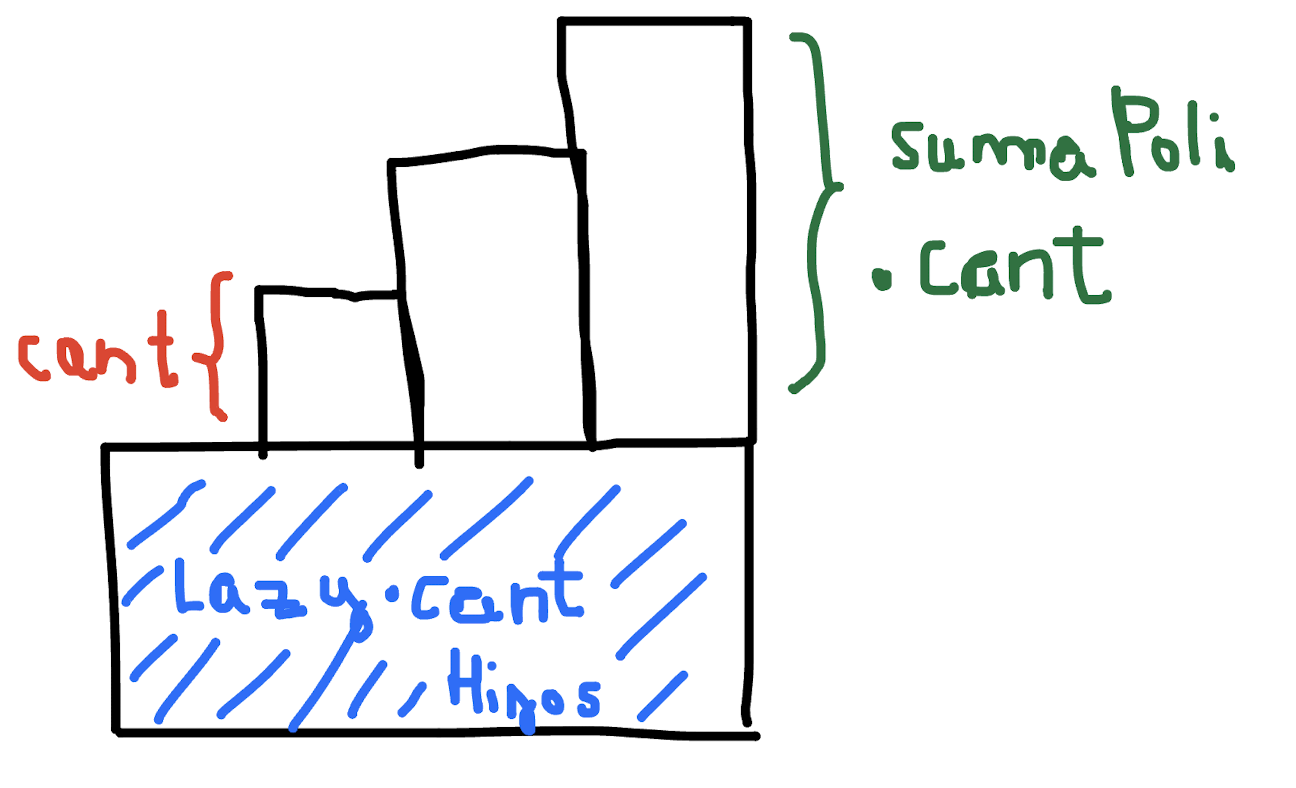
\includegraphics[width=0.3\linewidth]{grafico_poly_queries.png}
\end{center}

Ahora que sabemos los valores del nodo, debemos pensar el paso de propagación, el cuál no es tan sencillo ya que no es igual para el nodo izquierdo y para el nodo derecho. Para el nodo izquierdo, simplemente le sumamos tanto los valores $lazy$ como $cantidad$ del padre. Esto se debe a que el comienzo de la secuencia para la el hijo izquierdo es igual al comienzo de la secuencia para el nodo padre. Por ende, este nodo hijo va a abarcar un rango menor al padre, pero va a comenzar igual.

Para el nodo derecho, se le va a sumar $cantidad$ ya que ese es el número de operaciones (o la razón de la serie aritmética) que se le tiene que aplicar. Pero, $lazy$, que contiene el primer elemento de la secuencia, no se incrementa en $lazy$ del padre. En cambio, se lo incrementa por $temp = lazy + cantidad * mitadRangoActual$, siendo $mitadRangoActual = (r-l+1)/2$ y los tres valores haciendo referencia al nodo padre. Esto simplemente nos calcula el término de la sucesión en la posición $mitadRangoActual$, lo que hace que sea el primer término del subárbol derecho. De esta forma, podemos incrementar por $temp$ al valor $lazy$ del hijo derecho.

Por último, debemos notar que, al momento de actualizar un rango, cuando se recurre a los dos subárboles izquierdo y derecho luego de propagar, se hace hacia el nodo derecho con exactamente la misma división que en el paso de propagación, pero con la diferencia que toma como primera posición a la cantidad de nodos del subárbol derecho (que se puede calcular con $[l,r]$ y $[a,b]$ en la función recursiva). No entraré mucho en detalle ya que es similar al paso de propagación, y se puede ver en el código del Anexo.

De esta forma, quedó diseñada la estructura de datos para resolver el problema, por lo que solo resta leer el input y utilizarla. El problema resuelto quedará en el Anexo.

\section{Segment Tree Persistente}

Ahora, una pregunta motivadora que podemos hacernos es, ¿podemos hacer que las estructuras de datos viajen en el tiempo? Es decir, ¿podemos ir actualizando la estructura de datos y poder volver a visitar copias pasadas de la misma de forma eficiente, sin generar una copia cada vez? 

Una de las estructuras persistentes más simples son los \textit{arreglos persistentes}, que permiten en $O(1)$ agregar un elemento al arreglo y en $O(\log n)$ acceder al mismo en un tiempo $t$ determinado. Esto lo hace simplemente haciendo un arreglo de arreglo de pares, donde en cada arreglo se almacenan las tuplas $<tiempo,valor>$ para una posición determinada. Nosotros nos centraremos en ``Segment Trees'', que permitirán hacer consultas a lo largo de las distintas modificaciones. Muchas veces esto es explicado hablando de modificaciones a lo largo del tiempo, pero le daré un enfoque distinto: trabajaremos sobre hacer copias de la estructura de datos en tiempo y espacio $O(1)$, de tal forma que uno luego podrá modelar el ``tiempo'' de forma que sea necesaria, ya que podrá guardar las copias que uno quiera ya para los momentos que uno desee.

\subsection{Operaciones de la Estructura}

Esta estructura de datos soportará las siguientes operaciones:
\begin{itemize}
    \item \textit{query(l: int, r: int) -> int}: hacer una consulta de una operación en el ``Segment Tree''. Complejidad $O(\log n)$ tiempo, no modifica el espacio.
    \item \textit{update(pos: int, val: int)}: actualizar la posición $pos$ con el valor $val$. Complejidad $O(\log n)$ tiempo y espacio para cada llamada a la operación. Es decir, cada llamada a \textit{update} asignará $\log n$. Nuevas posiciones en memoria.
    \item \textit{copy()->PersistantSegmentTree}: genera una copia de la estructura de datos en $O(1)$. Modificar esta nueva estructura no modificará la anterior.

\end{itemize}

Para esta estructura de datos se puede utilizar cualquier Monoide.

\subsection{Representación de la Estructura}

Para representar la estructura, utilizaremos como base los ``Segment Trees Dinámicos'', es decir, los ``Segment Trees'' que viven en memoria dinámica. Cada estructura tendrá un nodo raíz $root$ que permitirá recorrerla, y cada nodo tendrá el valor del mismo, el puntero al hijo izquierdo y el puntero al hijo derecho. Veremos como trabajar con la estructura el la siguiente sección.

\subsection{Las Operaciones}

La operación \textit{query(l: int, r: int)} es idéntica a la del ``Segment Tree Dinámico'', no requiere ninguna modificación. Se utilizará la misma función auxiliar que el \textit{query} recursivo para la estructura clásica. 

La operación \textit{update(pos: int, val: int)} también será idéntica a la operación del ``Segment Tree Dinámico'', pero no se realizará la actualización sobre los nodos ya creados para esa estructura. En cambio, para cada uno de los $\log n$ nodos que se modificarán al momento de realizar una actualización, se crearán nuevos nodos. Para las ramas ya existentes y no modificadas, de todas formas, se apuntará a los nodos originales ya creados anteriormente. De esta forma, en cada actualización, se creará siempre una nueva raíz (que siempre es modificada) que permitirá recorrer la estructura luego de realizar los cambios. Esta será la nueva raíz del ``Segment Tree Persistente''. Como los nodos previos a la actualización se mantuvieron intactos, recorrerlos desde la raíz anterior nos permitiría recorrer la estructura previa. ¡Y así con todas las versiones anteriores si guardamos sus raíces! Y lo mejor de todo, sumamos por la operación solo $O(\log n)$ de memoria. Esa es la magia de la operación.

Por último, definimos la operación \textit{copy()->PersistantSegmentTree}, que lo único que hace es copiar la referencia al nodo raíz y devolver una nueva instancia de \textit{PersistantSegmentTree}, con el fin de mantener la modularidad. Cabe aclarar que en buenas prácticas, habría que limpiar los nodos que pierden todas las referencias hacia él, ya que C++ no lo maneja de forma automática. De todas formas, esto no se suele hacer en programación competitiva, ya que nos dan mucha memoria y nunca es necesario liberarla.

Estas son las operaciones, que con breves modificaciones sobre el ``Segment Tree Dinámico'' nos agregan la capacidad de, por un poco de memoria más, guardar el historial a medida que se va modificando la estructura de datos. El manejo de esta estructura de verá de forma mucho más clara a partir de su código, que veremos a partir de un problema clásico, a continuación.

\subsection{Problemas}

\subsubsection{CSES 1737 - Range Queries and Copies}

\begin{tcolorbox}
Tu tarea es mantener una lista de arreglos que inicialmente tiene un solo arreglo. Debes procesar los siguientes tipos de consultas:

\begin{enumerate}
    \item Establecer el valor $a$ en el arreglo $k$ como $x$.
    \item Calcular la suma de los valores en el rango $[a, b]$ en el arreglo $k$.
    \item Crear una copia del arreglo $k$ y agregarlo al final de la lista.
\end{enumerate}
\end{tcolorbox}

Para resolver el problema, podemos utilizar la estructura antes mencionada para el Monoide suma. Se puede mantener un arreglo $arr$ de punteros a \textit{PersistantSegmentTree}, donde $arr[k]$ representa al arreglo $k$ dado por el enunciado. En la posición $1$ se encuentra la estructura correspondiente al arreglo inicial. Luego, para hacer actualizaciones o consultas del tipo $1$ o $2$, se puede hacer la consulta en la estructura $arr[k]$. Por último, para hacer una copia, se puede llamar a \textit{copy()}, y el puntero de la copia agregarlo al final de $arr$. Como las primeras dos operaciones se hacen en complejidad $O(\log n)$ y la tercera en $O(1)$, la complejidad en peor caso será de $O(q \log n)$, suficiente para resolver el problema. El código se encuentra en el Anexo.

\section{Conclusiones}

A lo largo de esta monografía pudimos desarrollar la estructura de datos ``Segment Tree'', que nos permite realizar distintos tipos tipos de consultas sobre un arreglo de información (que puede ser implícito o explícito), con actualizaciones sobre los datos que se almacenan. Además, analizamos distintas técnicas y variantes de esta estructura que nos permitirán obtener ciertas flexibilidades o ventajas para poder resolver problemas más complejos.

\subsection{Problemas Adicionales}

Estos son algunos problemas que pueden servir para trabajar los conceptos que estuvimos trabajando:
\begin{itemize}
    \item Range Update Queries: \href{https://cses.fi/problemset/task/1651}{https://cses.fi/problemset/task/1651}
    \item List Removals: \href{https://cses.fi/problemset/task/1749}{https://cses.fi/problemset/task/1749}
    \item Distinct Value Queries: \href{https://cses.fi/problemset/task/1734}{https://cses.fi/problemset/task/1734}
    \item Prefix Sum Queries: \href{https://cses.fi/problemset/task/2166}{https://cses.fi/problemset/task/2166}
    \item Sumo: \href{https://juez.oia.unsam.edu.ar/task/123}{https://juez.oia.unsam.edu.ar/task/123}
    \item Clima: \href{https://juez.oia.unsam.edu.ar/task/35}{https://juez.oia.unsam.edu.ar/task/35}
    \item Mega Inversions: \href{https://open.kattis.com/problems/megainversions}{https://open.kattis.com/problems/megainversions}
    \item Contando puentes: \href{https://juez.oia.unsam.edu.ar/task/12}{https://juez.oia.unsam.edu.ar/task/12}
\end{itemize}

\subsection{Bibliografía}

Esta es la bilbliografía consultada para la realización de la monografía:
\begin{itemize}
    \item Competitive Programmer Handbook: \href{https://cses.fi/book/book.pdf}{https://cses.fi/book/book.pdf}
    \item Repositorio del Competitive Programmer Handbook: \href{https://github.com/pllk/cphb}{https://github.com/pllk/cphb}
    \item OIA Wiki: \href{http://www.oia.unsam.edu.ar/wp-content/uploads/2017/11/segment-tree.pdf}{http://www.oia.unsam.edu.ar/wp-content/uploads/2017/11/segment-tree.pdf}
    \item Wikipedia: \href{https://es.wikipedia.org/wiki/Monoide}{https://es.wikipedia.org/wiki/Monoide}
    \item USACO Guide: \href{https://usaco.guide}{https://usaco.guide}
    \item CP Algorithms: \href{https://cp-algorithms.com}{https://cp-algorithms.com}
\end{itemize}
Agredecimientos a Antti Laaksonen por los gráficos utilizados en el Competitive Programmer Handbook.

\subsection{Temas Adicionales}
Estos son algunos temas que se pueden consultar para ampliar el conocimiento del tema:

\begin{itemize}
    \item Fenwick Tree
    \item Segment Tree y Fenwick Tree 2D
    \item Segment Tree Lazy Creation + Lazy Update (codigo de USACO Guide)
\end{itemize}

\newpage

\section{Anexo}

\subsection{CSES 1648 - Dynamic Range Sum Queries - Recursivo}
Link al Problema: \href{https://cses.fi/problemset/task/1648}{https://cses.fi/problemset/task/1648}
\inputminted{c++}{Problemas/1Recursivo.cpp}

\subsection{CSES 1648 - Dynamic Range Sum Queries - Iterativo}
Link al Problema: \href{https://cses.fi/problemset/task/1648}{https://cses.fi/problemset/task/1648}
\inputminted{c++}{Problemas/1Iterativo.cpp}

\subsection{CSES 1649 - Dynamic Range Minimum Queries}
Link al Problema: \href{https://cses.fi/problemset/task/1649}{https://cses.fi/problemset/task/1649}
\inputminted{c++}{Problemas/2.cpp}

\subsection{CSES 1143 - Hotel Queries}
Link al problema: \href{https://cses.fi/problemset/task/1143}{https://cses.fi/problemset/task/1143}
\inputminted{c++}{Problemas/4.cpp}

\subsection{CSES 1144 - Salary Queries}
Link al problema: \href{https://cses.fi/problemset/task/1144}{https://cses.fi/problemset/task/1144}
\inputminted{c++}{Problemas/5.cpp}

\subsection{CSES 1144 - Salary Queries Dinámico}
Link al problema: \href{https://cses.fi/problemset/task/1144}{https://cses.fi/problemset/task/1144}
\inputminted{c++}{Problemas/5Dinamico.cpp}

\subsection{CSES 1735 - Range Updates and Sums}
Link al problema: \href{https://cses.fi/problemset/task/1735}{https://cses.fi/problemset/task/1735}
\inputminted{c++}{Problemas/6.cpp}

\subsection{CSES 1736 - Polinomial Queries}
Link al problema: \href{https://cses.fi/problemset/task/1736}{https://cses.fi/problemset/task/1736}
\inputminted{c++}{Problemas/7.cpp}

\subsection{CSES 1737 - Range Queries and Copies}
Link al problema: \href{https://cses.fi/problemset/task/1737}{https://cses.fi/problemset/task/1737}
\inputminted{c++}{Problemas/8.cpp}

\end{document}
